\documentclass[a4paper,11pt]{article}

% Kodovani (cestiny) v dokumentu: utf-8
%\usepackage[cp1250]{inputenc}	% Omezena stredoevropska kodova stranka, pouze MSW.
\usepackage[utf8]{inputenc}	% Doporucujeme pouzivat UTF-8 (unicode).

\usepackage[margin=2cm]{geometry}
\newtoks\jmenopraktika \newtoks\jmeno \newtoks\datum
\newtoks\obor \newtoks\skupina \newtoks\rocnik \newtoks\semestr
\newtoks\cisloulohy \newtoks\jmenoulohy
\newtoks\tlak \newtoks\teplota \newtoks\vlhkost

\jmenopraktika={Fyzikální praktikum 3}
\jmeno={Lukáš Lejdar}
\datum={13. května 2025}
\obor={F}
\skupina={Út 14:00}

\cisloulohy={5}
\jmenoulohy={Franck-Hertzův experiment}

%%%%%%%%%%% Uzitecne balicky:
\usepackage[czech]{babel}

\usepackage{graphicx}
\usepackage{amsmath}
\usepackage{xspace}
\usepackage{url}
\usepackage{indentfirst}
\usepackage{wrapfig}
\usepackage{xcolor}
\usepackage{subfig}
\usepackage{subcaption}
\usepackage{enumitem}
\usepackage{tikzsymbols}
\usepackage{newfloat}
\usepackage{siunitx}


\DeclareFloatingEnvironment[fileext=lof]{graph}
\captionsetup[graph]{labelformat=simple, labelsep=colon, name=Graf}

%%%%%% Zamezeni parchantu:
\widowpenalty 10000 \clubpenalty 10000 \displaywidowpenalty 10000
%%%%%% Parametry pro moznost vsazeni vetsiho poctu obrazku na stranku
\setcounter{topnumber}{3}	  % max. pocet floatu nahore (specifikace t)
\setcounter{bottomnumber}{3}	  % max. pocet floatu dole (specifikace b)
\setcounter{totalnumber}{6}	  % max. pocet floatu na strance celkem
\renewcommand\topfraction{0.9}	  % max podil stranky pro floaty nahore
\renewcommand\bottomfraction{0.9} % max podil stranky pro floaty dole
\renewcommand\textfraction{0.1}	  % min podil stranky, ktery musi obsahovat text
\intextsep=8mm \textfloatsep=8mm  %\intextsep pro ulozeni [h] floatu a \textfloatsep pro [b] or [t]

% Tecky za cisly sekci:
\renewcommand{\thesection}{\arabic{section}.}
\renewcommand{\thesubsection}{\thesection\arabic{subsection}.}
% Jednopismenna mezera mezi cislem a nazvem kapitoly:
\makeatletter \def\@seccntformat#1{\csname the#1\endcsname\hspace{1ex}} \makeatother
%
\newcommand{\vsn}[4]{\ensuremath{#1 =} #2(#3)\,#4}
\newcommand{\vrn}[6]{\ensuremath{#1 =} (#2 $\pm$ #3)\,#4 ($p=$ #5\,\%, $\nu=$ #6)}

\newcommand*\circled[1]{\tikz[baseline=(char.base)]{
		\node[shape=circle,draw,inner sep=1pt] (char) {#1};}}

%%%%%%%%%%%%%%%%%%%%%%%%%%%%%%%%%%%%%%%%%%%%%%%%%%%%%%%%%%%%%%%%%%%%%%%%%%%%%%%
% Zacatek dokumentu
%%%%%%%%%%%%%%%%%%%%%%%%%%%%%%%%%%%%%%%%%%%%%%%%%%%%%%%%%%%%%%%%%%%%%%%%%%%%%%%

\begin{document}

\thispagestyle{empty}

{
\begin{center}
\sf 
{\Large Ústav fyziky a technologií plazmatu Přírodovědecké fakulty Masarykovy univerzity} \\
\bigskip
{\huge \bfseries FYZIKÁLNÍ PRAKTIKUM} \\
\bigskip
{\Large \the\jmenopraktika}
\end{center}

\bigskip

\sf
\noindent
\setlength{\arrayrulewidth}{1pt}
\begin{tabular*}{\textwidth}{@{\extracolsep{\fill}} l l}
\large {\bfseries Zpracoval:}  \the\jmeno & \large  {\bfseries Naměřeno:} \the\datum\\[2mm]
\large  {\bfseries Obor:} \the\obor  \hspace{40mm}  {\bfseries Skupina:} \the\skupina %
&\large {\bfseries Testováno:}\\
\\
\hline
\end{tabular*}
}

\bigskip

{
\sf
\noindent \begin{tabular}{p{4cm} p{0.6\textwidth}}
\Large  Úloha č. {\bfseries \the\cisloulohy:} \par
\smallskip
&\Large \bfseries \the\jmenoulohy  \\[2mm]
\end{tabular}
}

\vskip1cm

\section{Úvod}

V roce 1914 Franck a Hertz experimentálně prokázali kvantování energetických hladin v atomech pomocí analýzy elektronových srážek s parami atomů rtuti. Cílem praktika je provést tento experiment s elektronkou naplněnou některým vzácným plynem a z naměřených dat zjistit o který jde plyn.

\section{Postup měření}

Experimentální uspořádání je schematicky znázorněno na obrázku 1. Z katody C jsou termoemisí uvolňované elektrony, které pak vlétají dovnitř elektronky naplněné některým vzácným plynem. V elektronce se nacházejí postupně dvě mřížky $ G_1 $ a $ G_2 $ a sběrná anoda. Pro experiment nejpodstatnější je urychlovací napětí mezi mřížkami $ G_1 $ a $ G_2 $ a brzdné napětí mezi mřížkou $ G_2 $ a anodou. Pokud mají elektrony při průletu mřížkou $ G_2 $ dostatečně velkou rychlost, dokáží brzdné napětí překonat a anodou začne téct měřitelný proud. V opačném případě si elektrony přitáhne mřížka $ G_2 $. 

\begin{figure}[htpb]
    \centering
    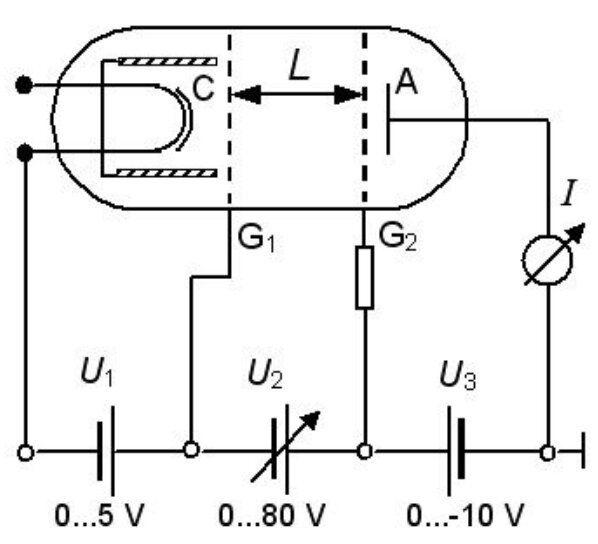
\includegraphics[width=0.4\textwidth]{zapojeni.jpg}
    \caption{Experimentální uspořádání Franck-Hertzova pokusu}
\end{figure}

%Elektrony jsou několika tisíci násobně lehčí než atomy, takže při pružné srážce se jen odrazí s minimální ztrátou kinetické energie podobně jako gumový míček odražený od bowlingové koule. Pokud je střední volná dráha elektronů dostatečně dlouhá, aby takových srážek nebylo moc 

Při zvyšování urychlovacího napětí by se dalo čekat, že proud jenom poroste až do nějaké hranice nasyceného proudu. Voltampérová charakteristika elektronky naplněné rtutí na Obrázku 2, naměřená Franck-Hertzem, ale namísto toho periodicky klesá ve stabilním intervalu přibližně $ \Delta U_2 = 4.9 $ V. Toto je známá hodnota energie jedné výrazné spektrální čáry rtuti, což naznačuje, že pokles proudu vzniká kvůli nepružným srážkám elektronů s atomy, kdy elektron ztratí velkou část své kinetické energie při excitaci a už není schopný překonat brzdné napětí. Tato hypotéza by měla být jednoduše ověřitelná, protože excitovaný atom sám od sebe brzo zase de-excituje a vyzáří foton o vlnové délce $ \lambda = hc / \Delta U_2 = 2530 \ \si{\angstrom}$. Na spektrometru by potom měla být vidět jediná spektrální čára o této vlnové délce. 


\begin{figure}[htpb]
    \centering
    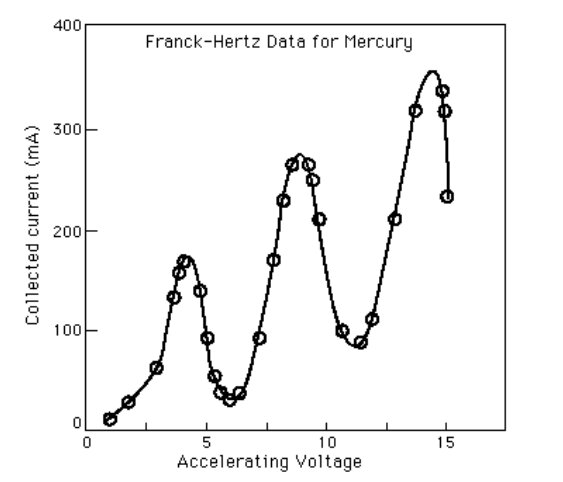
\includegraphics[width=0.4\textwidth]{hg.jpg}
    \caption{Závislost kolektorového proudu na urychlujícím napětí pro rtuť}
\end{figure}

 V uspořádání z obrázku 1. hraje roli ještě několik věcí. Urychlující napětí $ U_1 $ slouží ke stabilizaci měření, ale tím ovlivňuje první maximum. Kromě toho, elektron, který překoná první excitační energii ještě musí průměrně urazit jednu střední volnou dráhu, než se srazí s některým atomem a proto maxima nejsou ostrá a ani nenastávají v moment kdy energie elektronů přímo u mřížky $ G_2 $ dosáhne excitační energie $ \Delta E = e( U_1 + U_2 )$. Z těchto důvodů je lepší odečítat jen rozdíl po sobě následujících maxim $ \Delta U_2 $ a nedívat se na jeji absolutní velikosti. 

\section{Výsledky měření}

Experimentální aparatura byla sestavená podle Obrázku 1 s rozdílem, že místo anodového proudu se měří anodové napětí $ U_a \propto I_a $. Před měřením jsem nejdřív ověřil jestli všechny řídící napětí $ U_1 $, $ U_2 $ a $ U_3 $ fungují správně a potom hledal nejvhodnější nastavení napětí $ U_1 $ a $ U_3 $, aby maxima byli dobře vidět a zabírali co největší část měřícího rozsahu. Tyto hodnoty jsem nakonec našel jako $ U_1 = 2.36 $ V a $ U_3 = 9.91 $ V a pro ně změřil závislost $ U_a(U_2) $, která je vynesená do Grafu 1. 


\begin{figure}[htpb]
    \centering
    % GNUPLOT: LaTeX picture with Postscript
\begingroup
  \makeatletter
  \providecommand\color[2][]{%
    \GenericError{(gnuplot) \space\space\space\@spaces}{%
      Package color not loaded in conjunction with
      terminal option `colourtext'%
    }{See the gnuplot documentation for explanation.%
    }{Either use 'blacktext' in gnuplot or load the package
      color.sty in LaTeX.}%
    \renewcommand\color[2][]{}%
  }%
  \providecommand\includegraphics[2][]{%
    \GenericError{(gnuplot) \space\space\space\@spaces}{%
      Package graphicx or graphics not loaded%
    }{See the gnuplot documentation for explanation.%
    }{The gnuplot epslatex terminal needs graphicx.sty or graphics.sty.}%
    \renewcommand\includegraphics[2][]{}%
  }%
  \providecommand\rotatebox[2]{#2}%
  \@ifundefined{ifGPcolor}{%
    \newif\ifGPcolor
    \GPcolorfalse
  }{}%
  \@ifundefined{ifGPblacktext}{%
    \newif\ifGPblacktext
    \GPblacktexttrue
  }{}%
  % define a \g@addto@macro without @ in the name:
  \let\gplgaddtomacro\g@addto@macro
  % define empty templates for all commands taking text:
  \gdef\gplbacktext{}%
  \gdef\gplfronttext{}%
  \makeatother
  \ifGPblacktext
    % no textcolor at all
    \def\colorrgb#1{}%
    \def\colorgray#1{}%
  \else
    % gray or color?
    \ifGPcolor
      \def\colorrgb#1{\color[rgb]{#1}}%
      \def\colorgray#1{\color[gray]{#1}}%
      \expandafter\def\csname LTw\endcsname{\color{white}}%
      \expandafter\def\csname LTb\endcsname{\color{black}}%
      \expandafter\def\csname LTa\endcsname{\color{black}}%
      \expandafter\def\csname LT0\endcsname{\color[rgb]{1,0,0}}%
      \expandafter\def\csname LT1\endcsname{\color[rgb]{0,1,0}}%
      \expandafter\def\csname LT2\endcsname{\color[rgb]{0,0,1}}%
      \expandafter\def\csname LT3\endcsname{\color[rgb]{1,0,1}}%
      \expandafter\def\csname LT4\endcsname{\color[rgb]{0,1,1}}%
      \expandafter\def\csname LT5\endcsname{\color[rgb]{1,1,0}}%
      \expandafter\def\csname LT6\endcsname{\color[rgb]{0,0,0}}%
      \expandafter\def\csname LT7\endcsname{\color[rgb]{1,0.3,0}}%
      \expandafter\def\csname LT8\endcsname{\color[rgb]{0.5,0.5,0.5}}%
    \else
      % gray
      \def\colorrgb#1{\color{black}}%
      \def\colorgray#1{\color[gray]{#1}}%
      \expandafter\def\csname LTw\endcsname{\color{white}}%
      \expandafter\def\csname LTb\endcsname{\color{black}}%
      \expandafter\def\csname LTa\endcsname{\color{black}}%
      \expandafter\def\csname LT0\endcsname{\color{black}}%
      \expandafter\def\csname LT1\endcsname{\color{black}}%
      \expandafter\def\csname LT2\endcsname{\color{black}}%
      \expandafter\def\csname LT3\endcsname{\color{black}}%
      \expandafter\def\csname LT4\endcsname{\color{black}}%
      \expandafter\def\csname LT5\endcsname{\color{black}}%
      \expandafter\def\csname LT6\endcsname{\color{black}}%
      \expandafter\def\csname LT7\endcsname{\color{black}}%
      \expandafter\def\csname LT8\endcsname{\color{black}}%
    \fi
  \fi
    \setlength{\unitlength}{0.0500bp}%
    \ifx\gptboxheight\undefined%
      \newlength{\gptboxheight}%
      \newlength{\gptboxwidth}%
      \newsavebox{\gptboxtext}%
    \fi%
    \setlength{\fboxrule}{0.5pt}%
    \setlength{\fboxsep}{1pt}%
    \definecolor{tbcol}{rgb}{1,1,1}%
\begin{picture}(8640.00,5040.00)%
    \gplgaddtomacro\gplbacktext{%
      \csname LTb\endcsname%%
      \put(682,151){\makebox(0,0)[r]{\strut{}$10$}}%
      \put(682,929){\makebox(0,0)[r]{\strut{}$20$}}%
      \put(682,1707){\makebox(0,0)[r]{\strut{}$30$}}%
      \put(682,2485){\makebox(0,0)[r]{\strut{}$40$}}%
      \put(682,3263){\makebox(0,0)[r]{\strut{}$50$}}%
      \put(682,4041){\makebox(0,0)[r]{\strut{}$60$}}%
      \put(682,4819){\makebox(0,0)[r]{\strut{}$70$}}%
      \put(1726,-69){\makebox(0,0){\strut{}$2000$}}%
      \put(2812,-69){\makebox(0,0){\strut{}$2500$}}%
      \put(3899,-69){\makebox(0,0){\strut{}$3000$}}%
      \put(4985,-69){\makebox(0,0){\strut{}$3500$}}%
      \put(6071,-69){\makebox(0,0){\strut{}$4000$}}%
      \put(7157,-69){\makebox(0,0){\strut{}$4500$}}%
      \put(8243,-69){\makebox(0,0){\strut{}$5000$}}%
    }%
    \gplgaddtomacro\gplfronttext{%
      \csname LTb\endcsname%%
      \put(7256,4646){\makebox(0,0)[r]{\strut{}čidlo 1}}%
      \csname LTb\endcsname%%
      \put(7256,4426){\makebox(0,0)[r]{\strut{}čidlo 2}}%
      \csname LTb\endcsname%%
      \put(7256,4206){\makebox(0,0)[r]{\strut{}čidlo 3}}%
      \csname LTb\endcsname%%
      \put(7256,3986){\makebox(0,0)[r]{\strut{}čidlo 4}}%
      \csname LTb\endcsname%%
      \put(7256,3766){\makebox(0,0)[r]{\strut{}fit}}%
      \csname LTb\endcsname%%
      \put(209,2485){\rotatebox{-270.00}{\makebox(0,0){\strut{}t $^{\circ} C$}}}%
      \put(4528,-399){\makebox(0,0){\strut{}$\tau$ [s]}}%
    }%
    \gplbacktext
    \put(0,0){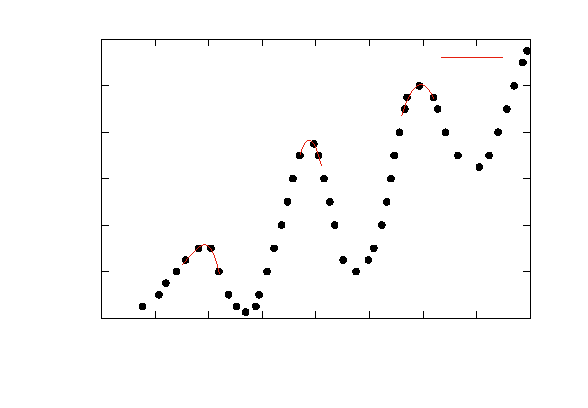
\includegraphics[width={432.00bp},height={252.00bp}]{mereni}}%
    \gplfronttext
  \end{picture}%
\endgroup

    \captionsetup{type=graph}
    \caption{Závislost anodového napětí na urychlujícím napětí $ U_2 $ }
\end{figure}

Data v okolí maxim byla nafitovaná polynomy řádu 5 a z nich jsem zjistil souřadnice lokálních maxim, které jsou uvedené v tabulce 1. Z fitu přímkou jsem potom získal sklon $ \Delta U_2 $. Takto vysokou první excitační energii má jenom Helium, která má velikost $ 19.8 $ eV. Druhá nejvyšší je první excitační energie Neonu, která je $ 16.6 $ eV  . 

\begin{equation}
\Delta U_2 = 20 \pm 0.6 \text{ eV}
\end{equation}


\begin{table}[htpb]
    \begin{minipage}{.4\linewidth}
        \centering
        \begin{tabular}{| c c c |}
            \hline
            maximum & $ U_2 $ (V) & $ U_a $ (V)  \\
            \hline
            1 & 22.0 & 3.15 \\
            2 & 41.0 & 7.65 \\
            3 & 62.0 & 10.1 \\
            \hline
        \end{tabular}
        \caption{Hodnoty lokálních maxim}
    \end{minipage} 
    \hfill
    \begin{minipage}{.55\linewidth}
        \centering
        \resizebox{\textwidth}{!}{ % GNUPLOT: LaTeX picture with Postscript
\begingroup
  \makeatletter
  \providecommand\color[2][]{%
    \GenericError{(gnuplot) \space\space\space\@spaces}{%
      Package color not loaded in conjunction with
      terminal option `colourtext'%
    }{See the gnuplot documentation for explanation.%
    }{Either use 'blacktext' in gnuplot or load the package
      color.sty in LaTeX.}%
    \renewcommand\color[2][]{}%
  }%
  \providecommand\includegraphics[2][]{%
    \GenericError{(gnuplot) \space\space\space\@spaces}{%
      Package graphicx or graphics not loaded%
    }{See the gnuplot documentation for explanation.%
    }{The gnuplot epslatex terminal needs graphicx.sty or graphics.sty.}%
    \renewcommand\includegraphics[2][]{}%
  }%
  \providecommand\rotatebox[2]{#2}%
  \@ifundefined{ifGPcolor}{%
    \newif\ifGPcolor
    \GPcolorfalse
  }{}%
  \@ifundefined{ifGPblacktext}{%
    \newif\ifGPblacktext
    \GPblacktexttrue
  }{}%
  % define a \g@addto@macro without @ in the name:
  \let\gplgaddtomacro\g@addto@macro
  % define empty templates for all commands taking text:
  \gdef\gplbacktext{}%
  \gdef\gplfronttext{}%
  \makeatother
  \ifGPblacktext
    % no textcolor at all
    \def\colorrgb#1{}%
    \def\colorgray#1{}%
  \else
    % gray or color?
    \ifGPcolor
      \def\colorrgb#1{\color[rgb]{#1}}%
      \def\colorgray#1{\color[gray]{#1}}%
      \expandafter\def\csname LTw\endcsname{\color{white}}%
      \expandafter\def\csname LTb\endcsname{\color{black}}%
      \expandafter\def\csname LTa\endcsname{\color{black}}%
      \expandafter\def\csname LT0\endcsname{\color[rgb]{1,0,0}}%
      \expandafter\def\csname LT1\endcsname{\color[rgb]{0,1,0}}%
      \expandafter\def\csname LT2\endcsname{\color[rgb]{0,0,1}}%
      \expandafter\def\csname LT3\endcsname{\color[rgb]{1,0,1}}%
      \expandafter\def\csname LT4\endcsname{\color[rgb]{0,1,1}}%
      \expandafter\def\csname LT5\endcsname{\color[rgb]{1,1,0}}%
      \expandafter\def\csname LT6\endcsname{\color[rgb]{0,0,0}}%
      \expandafter\def\csname LT7\endcsname{\color[rgb]{1,0.3,0}}%
      \expandafter\def\csname LT8\endcsname{\color[rgb]{0.5,0.5,0.5}}%
    \else
      % gray
      \def\colorrgb#1{\color{black}}%
      \def\colorgray#1{\color[gray]{#1}}%
      \expandafter\def\csname LTw\endcsname{\color{white}}%
      \expandafter\def\csname LTb\endcsname{\color{black}}%
      \expandafter\def\csname LTa\endcsname{\color{black}}%
      \expandafter\def\csname LT0\endcsname{\color{black}}%
      \expandafter\def\csname LT1\endcsname{\color{black}}%
      \expandafter\def\csname LT2\endcsname{\color{black}}%
      \expandafter\def\csname LT3\endcsname{\color{black}}%
      \expandafter\def\csname LT4\endcsname{\color{black}}%
      \expandafter\def\csname LT5\endcsname{\color{black}}%
      \expandafter\def\csname LT6\endcsname{\color{black}}%
      \expandafter\def\csname LT7\endcsname{\color{black}}%
      \expandafter\def\csname LT8\endcsname{\color{black}}%
    \fi
  \fi
    \setlength{\unitlength}{0.0500bp}%
    \ifx\gptboxheight\undefined%
      \newlength{\gptboxheight}%
      \newlength{\gptboxwidth}%
      \newsavebox{\gptboxtext}%
    \fi%
    \setlength{\fboxrule}{0.5pt}%
    \setlength{\fboxsep}{1pt}%
    \definecolor{tbcol}{rgb}{1,1,1}%
\begin{picture}(5328.00,3600.00)%
    \gplgaddtomacro\gplbacktext{%
      \csname LTb\endcsname%%
      \put(682,834){\makebox(0,0)[r]{\strut{}$20$}}%
      \put(682,1391){\makebox(0,0)[r]{\strut{}$30$}}%
      \put(682,1949){\makebox(0,0)[r]{\strut{}$40$}}%
      \put(682,2506){\makebox(0,0)[r]{\strut{}$50$}}%
      \put(682,3063){\makebox(0,0)[r]{\strut{}$60$}}%
      \put(1157,484){\makebox(0,0){\strut{}$1$}}%
      \put(2872,484){\makebox(0,0){\strut{}$2$}}%
      \put(4588,484){\makebox(0,0){\strut{}$3$}}%
    }%
    \gplgaddtomacro\gplfronttext{%
      \csname LTb\endcsname%%
      \put(209,2041){\rotatebox{-270}{\makebox(0,0){\strut{}$ U_2 $ (V)}}}%
      \put(2872,154){\makebox(0,0){\strut{}Násobnost maxima}}%
      \csname LTb\endcsname%%
      \put(2429,3109){\makebox(0,0)[r]{\strut{}fit $ \Delta U_2 x + U_{20} $}}%
    }%
    \gplbacktext
    \put(0,0){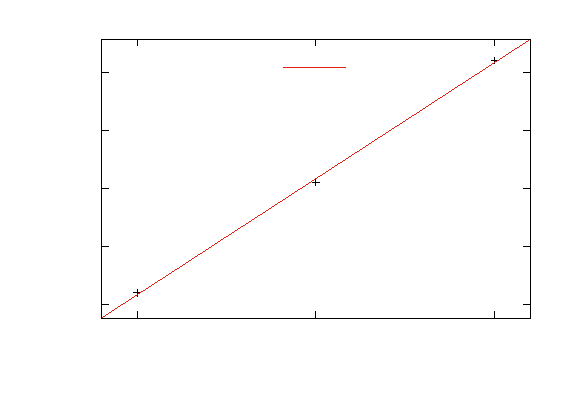
\includegraphics[width={266.40bp},height={180.00bp}]{peaks}}%
    \gplfronttext
  \end{picture}%
\endgroup
 }
        \caption{}
    \end{minipage} 
\end{table}

\subsection{Emitované spektrum}

V praktiku se k úloze nachází příruční spektrometr, kterým jsem změřil spektrum vyzařované z trubice Franck-Hertzova experimentu a výsledné hodnoty vynesl do grafu 2. Pokud je efekt způsobený jediným přechodem, měla by na spektrometru být vidět pouze jedna čára o vlnové délce $ \lambda = hc / \Delta U_2 = 62 $ nm, nebo potažmo žádná protože spektrometr nemá dostatečný rozsah. Je ale vidět, že se ve spektru nachází podstatně víc čar, takže změřený rozdíl maxim $ \Delta U_2 $ pravděpodobně neodpovídá žádné jedné excitační energii. Na druhou stranu víme, že $ \Delta U_2 $ nemůže být větší než ionizační energie plynu, což možnosti redukuje na Helium, nebo Neon. Známé vlnové délky jsem zjistil z odkazu [2] a vynesl je do Grafu 2 společně se změřeným spektrem. Je vidět, že na data sedí mnohem líp spektrum Neonu. Nejintenzivnější čára ve spektru má vlnovou délku $ \lambda \approx 585 $ nm, která odpovídá přechodu $ 2s^22p^{5}3p \to  2s^22p^{5}3s $ a její energie je $ \Delta E = hc / \lambda = 2.11 $ eV. 

\vspace{-1pt}

\begin{figure}[htpb]
    \centering
    % GNUPLOT: LaTeX picture with Postscript
\begingroup
  \makeatletter
  \providecommand\color[2][]{%
    \GenericError{(gnuplot) \space\space\space\@spaces}{%
      Package color not loaded in conjunction with
      terminal option `colourtext'%
    }{See the gnuplot documentation for explanation.%
    }{Either use 'blacktext' in gnuplot or load the package
      color.sty in LaTeX.}%
    \renewcommand\color[2][]{}%
  }%
  \providecommand\includegraphics[2][]{%
    \GenericError{(gnuplot) \space\space\space\@spaces}{%
      Package graphicx or graphics not loaded%
    }{See the gnuplot documentation for explanation.%
    }{The gnuplot epslatex terminal needs graphicx.sty or graphics.sty.}%
    \renewcommand\includegraphics[2][]{}%
  }%
  \providecommand\rotatebox[2]{#2}%
  \@ifundefined{ifGPcolor}{%
    \newif\ifGPcolor
    \GPcolorfalse
  }{}%
  \@ifundefined{ifGPblacktext}{%
    \newif\ifGPblacktext
    \GPblacktexttrue
  }{}%
  % define a \g@addto@macro without @ in the name:
  \let\gplgaddtomacro\g@addto@macro
  % define empty templates for all commands taking text:
  \gdef\gplbacktext{}%
  \gdef\gplfronttext{}%
  \makeatother
  \ifGPblacktext
    % no textcolor at all
    \def\colorrgb#1{}%
    \def\colorgray#1{}%
  \else
    % gray or color?
    \ifGPcolor
      \def\colorrgb#1{\color[rgb]{#1}}%
      \def\colorgray#1{\color[gray]{#1}}%
      \expandafter\def\csname LTw\endcsname{\color{white}}%
      \expandafter\def\csname LTb\endcsname{\color{black}}%
      \expandafter\def\csname LTa\endcsname{\color{black}}%
      \expandafter\def\csname LT0\endcsname{\color[rgb]{1,0,0}}%
      \expandafter\def\csname LT1\endcsname{\color[rgb]{0,1,0}}%
      \expandafter\def\csname LT2\endcsname{\color[rgb]{0,0,1}}%
      \expandafter\def\csname LT3\endcsname{\color[rgb]{1,0,1}}%
      \expandafter\def\csname LT4\endcsname{\color[rgb]{0,1,1}}%
      \expandafter\def\csname LT5\endcsname{\color[rgb]{1,1,0}}%
      \expandafter\def\csname LT6\endcsname{\color[rgb]{0,0,0}}%
      \expandafter\def\csname LT7\endcsname{\color[rgb]{1,0.3,0}}%
      \expandafter\def\csname LT8\endcsname{\color[rgb]{0.5,0.5,0.5}}%
    \else
      % gray
      \def\colorrgb#1{\color{black}}%
      \def\colorgray#1{\color[gray]{#1}}%
      \expandafter\def\csname LTw\endcsname{\color{white}}%
      \expandafter\def\csname LTb\endcsname{\color{black}}%
      \expandafter\def\csname LTa\endcsname{\color{black}}%
      \expandafter\def\csname LT0\endcsname{\color{black}}%
      \expandafter\def\csname LT1\endcsname{\color{black}}%
      \expandafter\def\csname LT2\endcsname{\color{black}}%
      \expandafter\def\csname LT3\endcsname{\color{black}}%
      \expandafter\def\csname LT4\endcsname{\color{black}}%
      \expandafter\def\csname LT5\endcsname{\color{black}}%
      \expandafter\def\csname LT6\endcsname{\color{black}}%
      \expandafter\def\csname LT7\endcsname{\color{black}}%
      \expandafter\def\csname LT8\endcsname{\color{black}}%
    \fi
  \fi
    \setlength{\unitlength}{0.0500bp}%
    \ifx\gptboxheight\undefined%
      \newlength{\gptboxheight}%
      \newlength{\gptboxwidth}%
      \newsavebox{\gptboxtext}%
    \fi%
    \setlength{\fboxrule}{0.5pt}%
    \setlength{\fboxsep}{1pt}%
    \definecolor{tbcol}{rgb}{1,1,1}%
\begin{picture}(9936.00,3600.00)%
    \gplgaddtomacro\gplbacktext{%
      \csname LTb\endcsname%%
      \put(858,440){\makebox(0,0)[r]{\strut{}$0$}}%
      \put(858,1028){\makebox(0,0)[r]{\strut{}$2000$}}%
      \put(858,1616){\makebox(0,0)[r]{\strut{}$4000$}}%
      \put(858,2203){\makebox(0,0)[r]{\strut{}$6000$}}%
      \put(858,2791){\makebox(0,0)[r]{\strut{}$8000$}}%
      \put(858,3379){\makebox(0,0)[r]{\strut{}$10000$}}%
      \put(990,220){\makebox(0,0){\strut{}$515$}}%
      \put(1367,220){\makebox(0,0){\strut{}$525$}}%
      \put(1743,220){\makebox(0,0){\strut{}$535$}}%
      \put(2120,220){\makebox(0,0){\strut{}$545$}}%
      \put(2496,220){\makebox(0,0){\strut{}$555$}}%
      \put(2873,220){\makebox(0,0){\strut{}$565$}}%
      \put(3250,220){\makebox(0,0){\strut{}$575$}}%
      \put(3626,220){\makebox(0,0){\strut{}$585$}}%
      \put(4003,220){\makebox(0,0){\strut{}$595$}}%
      \put(4379,220){\makebox(0,0){\strut{}$605$}}%
      \put(4756,220){\makebox(0,0){\strut{}$615$}}%
      \put(5133,220){\makebox(0,0){\strut{}$625$}}%
      \put(5509,220){\makebox(0,0){\strut{}$635$}}%
      \put(5886,220){\makebox(0,0){\strut{}$645$}}%
      \put(6263,220){\makebox(0,0){\strut{}$655$}}%
      \put(6639,220){\makebox(0,0){\strut{}$665$}}%
      \put(7016,220){\makebox(0,0){\strut{}$675$}}%
      \put(7392,220){\makebox(0,0){\strut{}$685$}}%
      \put(7769,220){\makebox(0,0){\strut{}$695$}}%
      \put(8146,220){\makebox(0,0){\strut{}$705$}}%
      \put(8522,220){\makebox(0,0){\strut{}$715$}}%
      \put(8899,220){\makebox(0,0){\strut{}$725$}}%
      \put(9275,220){\makebox(0,0){\strut{}$735$}}%
    }%
    \gplgaddtomacro\gplfronttext{%
      \csname LTb\endcsname%%
      \put(99,1909){\rotatebox{-270}{\makebox(0,0){\strut{}}}}%
      \put(5264,-66){\makebox(0,0){\strut{}}}%
      \csname LTb\endcsname%%
      \put(3213,3181){\makebox(0,0)[r]{\strut{} spektrální čáry Neonu}}%
      \csname LTb\endcsname%%
      \put(3213,2961){\makebox(0,0)[r]{\strut{} spektrální čáry Helia}}%
    }%
    \gplbacktext
    \put(0,0){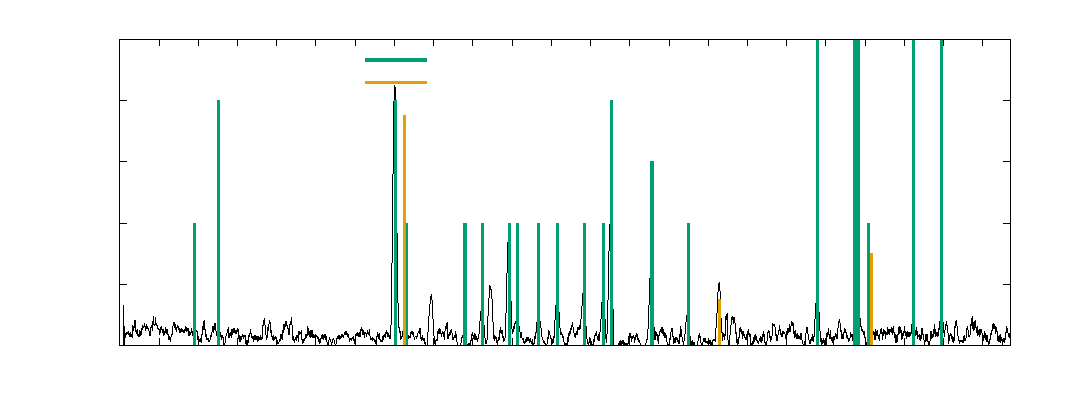
\includegraphics[width={496.80bp},height={180.00bp}]{spektrum}}%
    \gplfronttext
  \end{picture}%
\endgroup

    \captionsetup{type=graph}
    \caption{Spektrální závislost plynu v trubici}
\end{figure}

\section{Závěr}

Změřil jsem závislost anodového napětí na urychlovacím napětí v trubici Franck-Hertzova experimentu a zjistil, že se maxima opakují s periodou $ \Delta U_2 = 20 \pm 0.6 \text{ eV} $, což je hodnota, která by odpovídala první excitační energii Helia, která je $ 19.8 $ eV. Ze spektrální závislost ale vyplynulo, že neměříme jedinou spektrální čáru, ale celé spektrum, které odpovídá atomům Neonu. Ten má první excitační energii $ 16.6 $ eV. Z měření ale stále vyplývá, že existuje nějaká minimální energie, kterou může atom Neonu přijmout při excitaci do vyššího stavu.  

\begin{thebibliography}{0}
\bibitem{tabulky} Návod k úloze ~\url{https://is.muni.cz/auth/el/sci/jaro2025/F4210/um/fp3-5_Franck-Hertz.pdf}.   
\bibitem{spectra} Atomic spectra database  \\ ~\url{https://www.nist.gov/pml/productsservices/physical-reference-data}.   
\end{thebibliography}

\end{document}
